\listfiles
\documentclass[
    fontsize=11pt,%Schriftgröße
    paper=a4,%Papiergröße
    headings=small,
    parskip=half,
    listof=totoc,
    bibliography=totoc,
    pagesize
]{scrbook}
%\usepackage{scrhack}

\usepackage[utf8]{inputenc}
\usepackage[T1]{fontenc}
% Paket für Sprachen
\usepackage[ngerman]{babel}
\usepackage{libertine}
\usepackage[scaled=0.8]{beramono}
\usepackage{textcomp}
\usepackage{amsfonts} %dsfont
\usepackage{microtype}

\usepackage{geometry}
\geometry{inner=2cm,outer=4cm,top=2cm,bottom=4cm}

\usepackage[onehalfspacing]{setspace}

%\renewcommand{\familydefault}{\sfdefault}
\usepackage{blindtext}
\usepackage[newcommands]{ragged2e}
\usepackage{enumitem}
\newlist{exercise}{enumerate}{1}
\setlist[exercise]{label=(\alph*),font=\itshape,noitemsep}

\usepackage[headsepline]{scrpage2}
\clearscrheadfoot
\ohead{\pagemark}
\ihead{\headmark}
%\cfoot[Version vom \today]{Version vom \today}
\pagestyle{scrheadings}

\usepackage[]{floatrow}
\floatplacement{figure}{htb}
\floatplacement{table}{htb}
\floatsetup[table]{style=plaintop}
\DeclareNewFloatType{diagram}{
    name=Diagramm,
    placement=htb,
    fileext=lod,
    within=chapter
    }

\usepackage[hyperref,table,rgb,dvipsnames]{xcolor}

\usepackage[mark]{gitinfo2}
\renewcommand{\gitMark}{%
    Branch: \gitBranch\,@\,\gitAbbrevHash{}\textbullet{}Release:\gitReln{} (\gitAuthorDate)\\
    Head tags: \gitTags\\
    Autor: \gitCommitterName
}

\usepackage{graphicx}
\usepackage{subfig}
\usepackage{array}
\usepackage{booktabs}
\usepackage{tabularx}

\usepackage{siunitx}
\usepackage{amsmath}
\usepackage{amsthm}
\newtheoremstyle{break}%
{}{}%
{}{}%
{\bfseries}{}% % Note that final punctuation is omitted.
{\newline}{}

\theoremstyle{break}
\newtheorem{definition}{Definition}[chapter]
\theoremstyle{plain}
\newtheorem{satz}{Satz}[chapter]

\usepackage{mathtools}
\usepackage{chngcntr}
\counterwithout{equation}{chapter}

\usepackage{biblatex}
\addbibresource{LaTeX-Literatur.bib}
\usepackage{calc}
\usepackage[german]{varioref}
\usepackage[german]{cleveref}

\setkomafont{disposition}{\normalfont\bfseries}
\setkomafont{pagehead}{\normalfont\upshape\small}
\setkomafont{pagenumber}{\normalfont\bfseries\normalsize}
\setkomafont{caption}{\normalfont\small\itshape}
\setkomafont{captionlabel}{\normalfont\small\upshape\bfseries}


\deffootnote[1.5em]{1.5em}{1.5em}{\makebox[1.5em][r]{\textsuperscript{\footnotemark}\ }}

\newcommand{\autor}[1]{\textit{#1}} %-> \autor{Name}

\newenvironment{zitat}% ->\begin{zitat}...\end{zitat}
    {\par\vspace{5mm}\begin{addmargin}{1cm}\itshape\small}%
    {\end{addmargin}\par\vspace{5mm}}%


\begin{document}
\frontmatter
\title{Ein erstes Dokument mit \TeX{}}
\author{Martin Sievers\and N.N. \and X.Y.}
\date{}
\maketitle

\begin{spacing}{1.0}
\tableofcontents
\listoffigures
\listoftables
\listof{diagram}{Diagrammverzeichnis}
\end{spacing}

\mainmatter
\chapter{Aller Anfang ist schwer}\label{chap:AllerAnfang}
In Abschnitt~\ref{sec:ProblemeUmlaute} auf S.~\pageref{sec:ProblemeUmlaute}

In Abschnitt~\vref{sec:ProblemeUmlaute}
\blindtext[8]

\section{Probleme mit Umlauten}\label{sec:ProblemeUmlaute}
{\itshape   In der Kürze liegt die Würze.}
    
{\Large Ein \textbf{Sprichwort} besagt: "`5\,\% sind weniger 10\,\%"' Ein Sprichwort besagt: "`5\,\% sind 
weniger 10\,\%"' 
Ein 
Sprichwort besagt: "`5\,\% sind weniger 10\,\%"' Ein Sprichwort besagt: "`5\,\% sind weniger als 10\,\%"'}

\section{Das Spatium ("`halbes Leerzeichen"')}\label{sec:Spatium}
5\%\par 5\,\%

5~\%\\
z.B.\\
z.\,B.\\[2cm]
z.~B.

\chapter{Viel Blindtext}
Wie bereits in Kapitel~\ref{chap:AllerAnfang} auf S.~\pageref{chap:AllerAnfang} beschrieben

Wie bereits in \cref{sec:Spatium,chap:AllerAnfang,sec:ProblemeUmlaute}

\blindtext
\begin{center}
    \blindtext[2]
\end{center}
\blindtext[8]

\section{Fußnoten}
Ein wichtiger\footnote{vielleicht doch nicht.\par\blindtext} Text

\section{Listen}
\blindtext
\begin{itemize}[label=\textendash]
    \item Leicht
    \item Schwierig
    \begin{exercise}
        \item Prüfen Sie \ldots{}
        \item Testen Sie \ldots{}
    \end{exercise}
    \item Sehr schwierig
\end{itemize}

\subsection{Eigene Befehle}
Wie bereits der Autor \autor{Herbert Voß} schreibt: \blindtext

\autor{Markus Kohm} ist der Vater von KOMA-Script. Er schreibt:
\begin{zitat}
    \blindtext
\end{zitat}

\chapter{Tag 2}
\section{Floatobjekte}
\blindtext
\begin{figure}
    \centering
    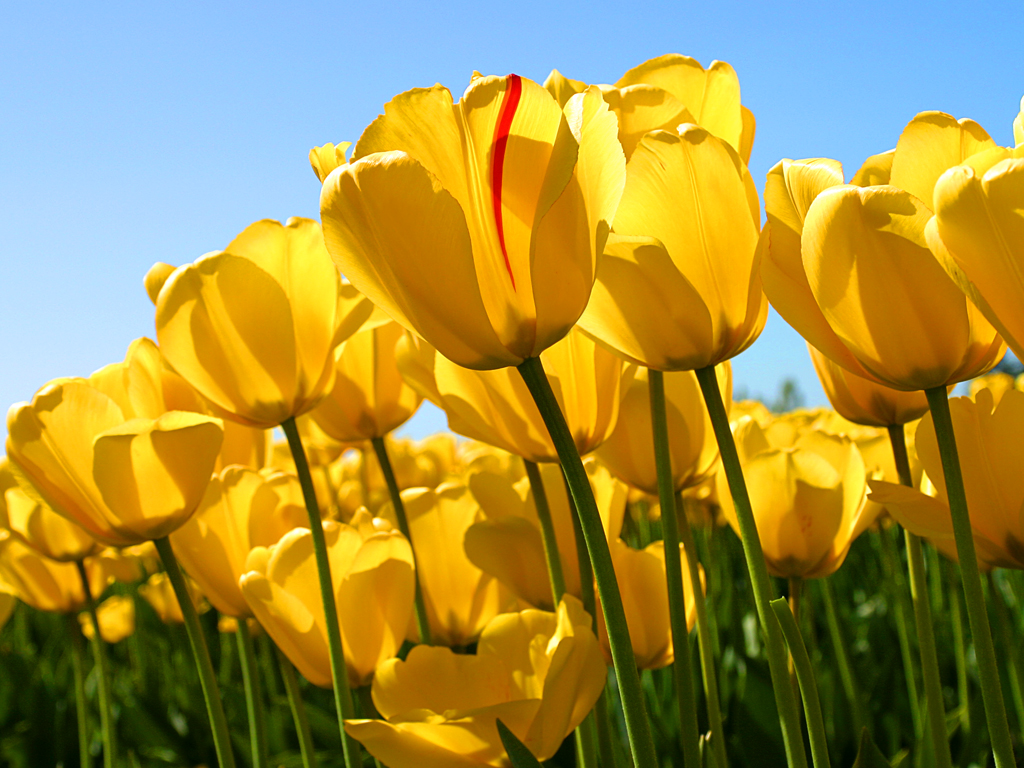
\includegraphics[width=6cm,height=8cm,keepaspectratio]{Abbildungen/Tulips}
    \caption[Tolle Abbildung]{Eine erste ganz tolle noch leere Abbildung}
    \label{fig:tolleAbbildung}
\end{figure}

\blindtext[3]
\begin{diagram}
    \caption{Ein erstes Diagramm}
    \label{diag:erstesDiagramm}
\end{diagram}

\blindtext[2]
\begin{figure}
    \centering
    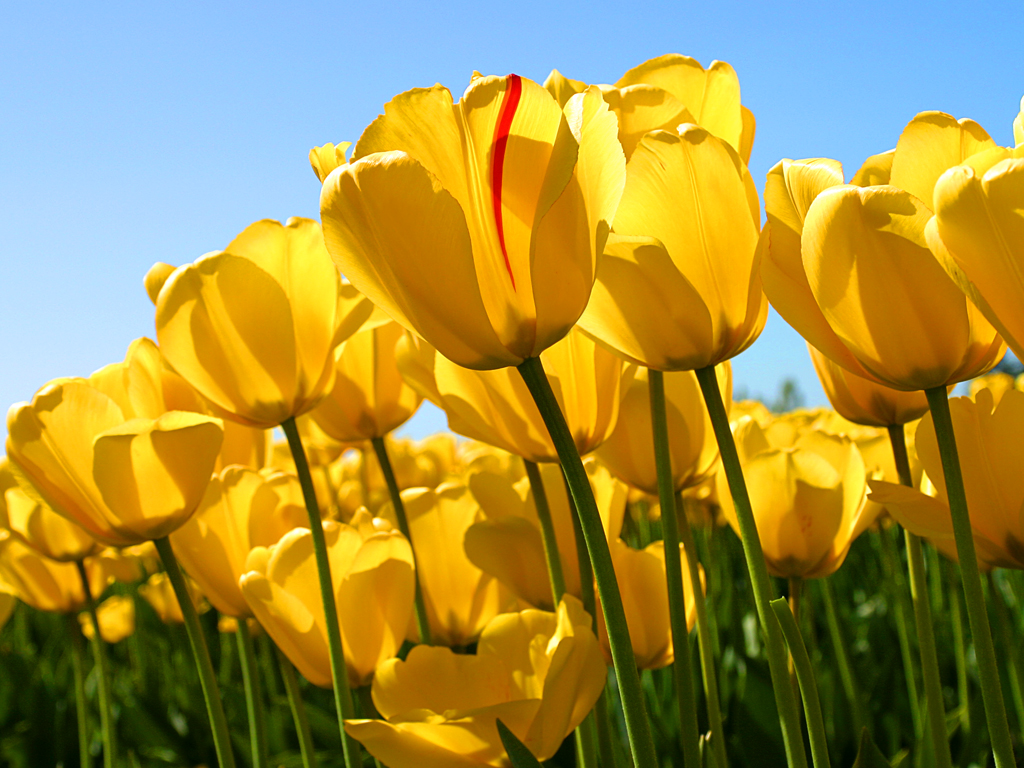
\includegraphics[width=0.85\linewidth]{Abbildungen/Tulips}
    \caption{Eine ganz tolle Abbildung}
    \label{fig:tolleAbbildung2}
\end{figure}

\blindtext[2]
\begin{figure}
\subfloat[Eine gelbe Tulpe]{
    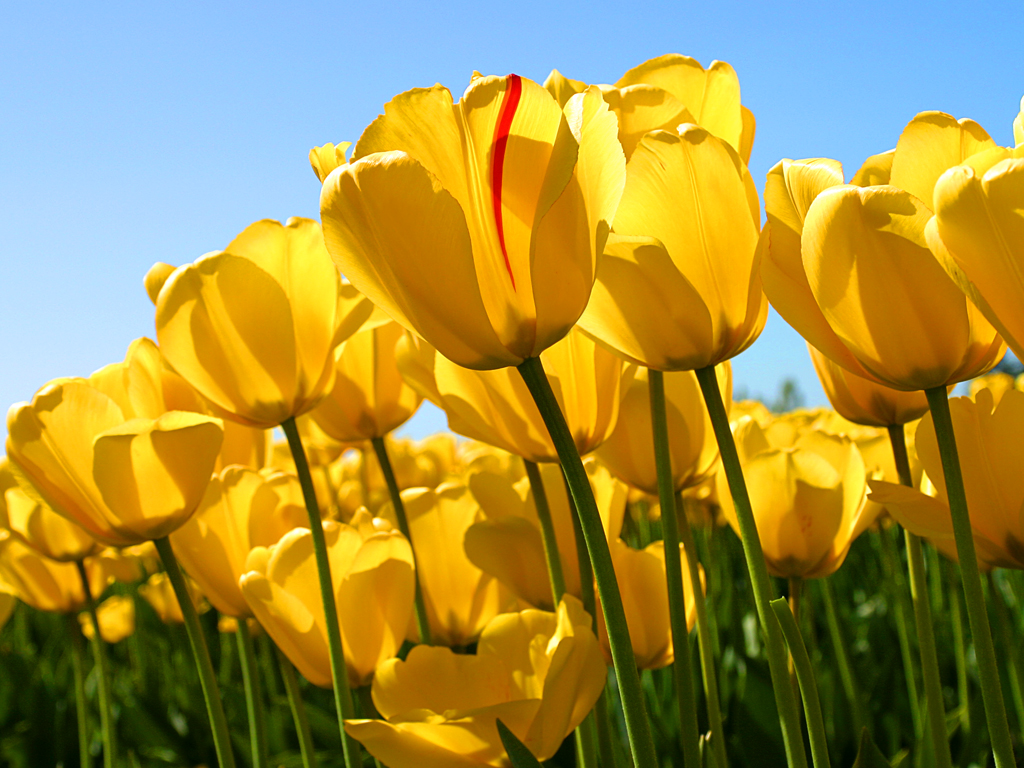
\includegraphics[width=0.45\linewidth]{Abbildungen/Tulips}}
\hfill
\subfloat[Der Kölner Dom von oben]{
    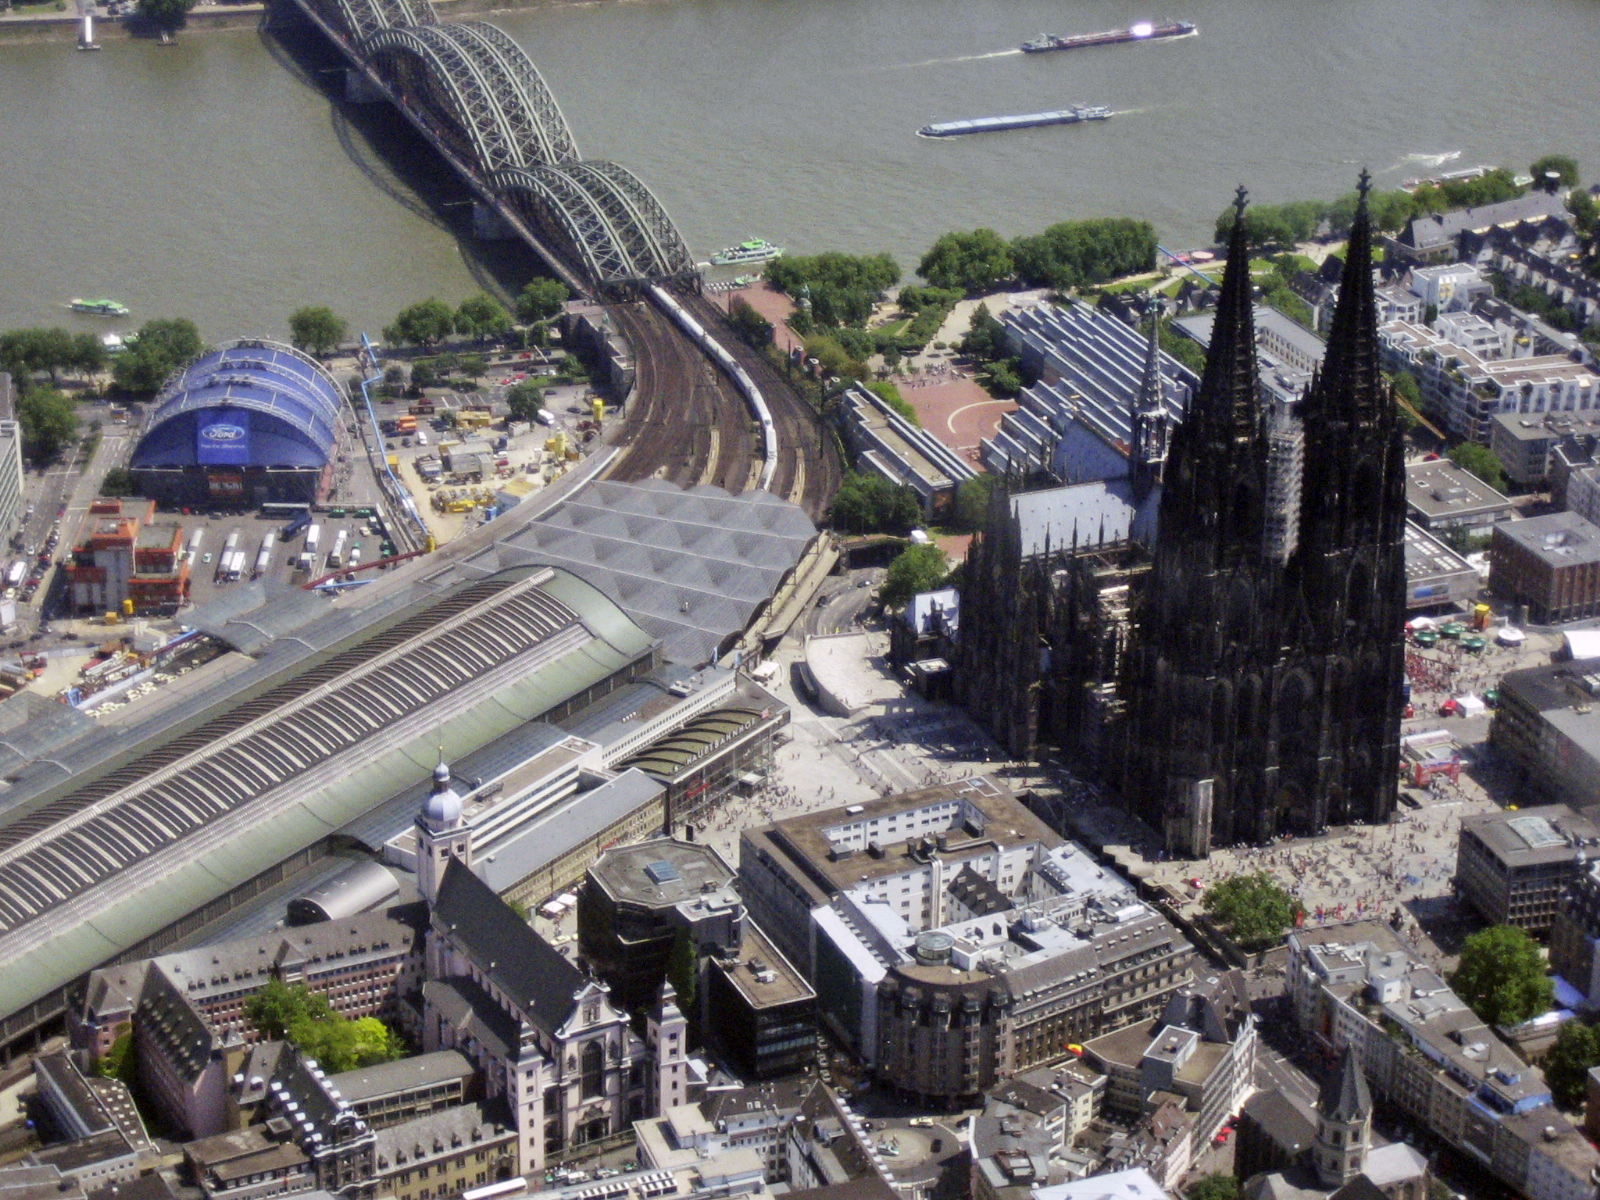
\includegraphics[width=0.45\linewidth]{Abbildungen/Koeln_RdFlug_1}}
\\
\subfloat[Eine gelbe Tulpe]{
    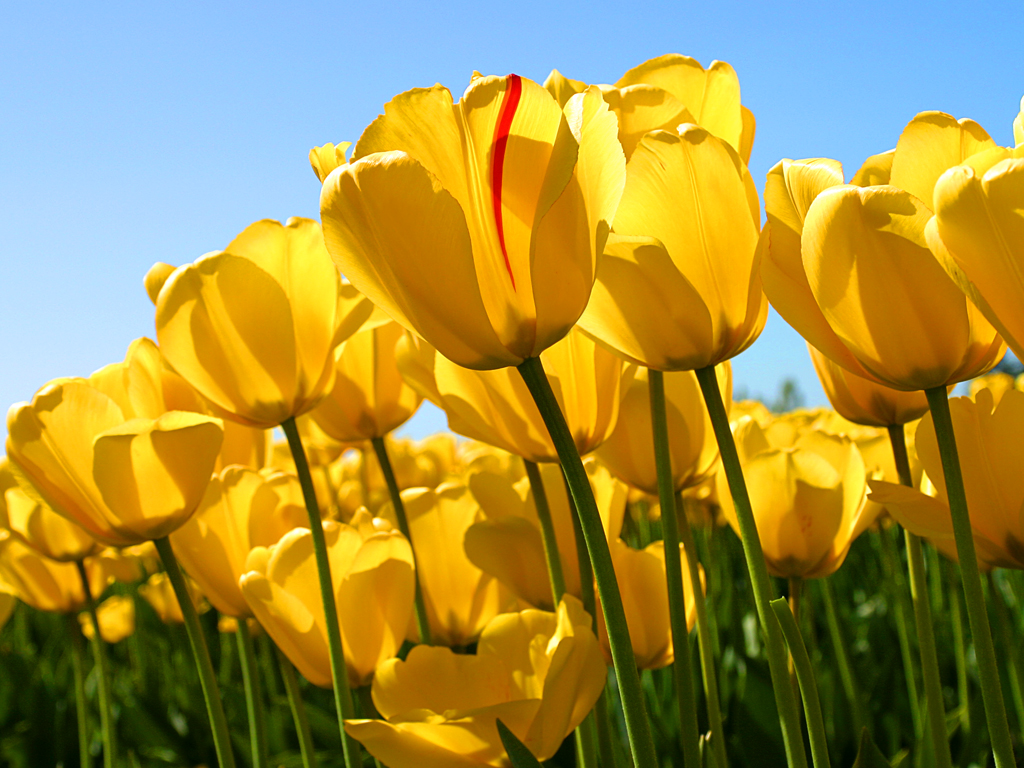
\includegraphics[width=0.45\linewidth]{Abbildungen/Tulips}}
\hfill
\subfloat[Der Kölner Dom von oben]{
    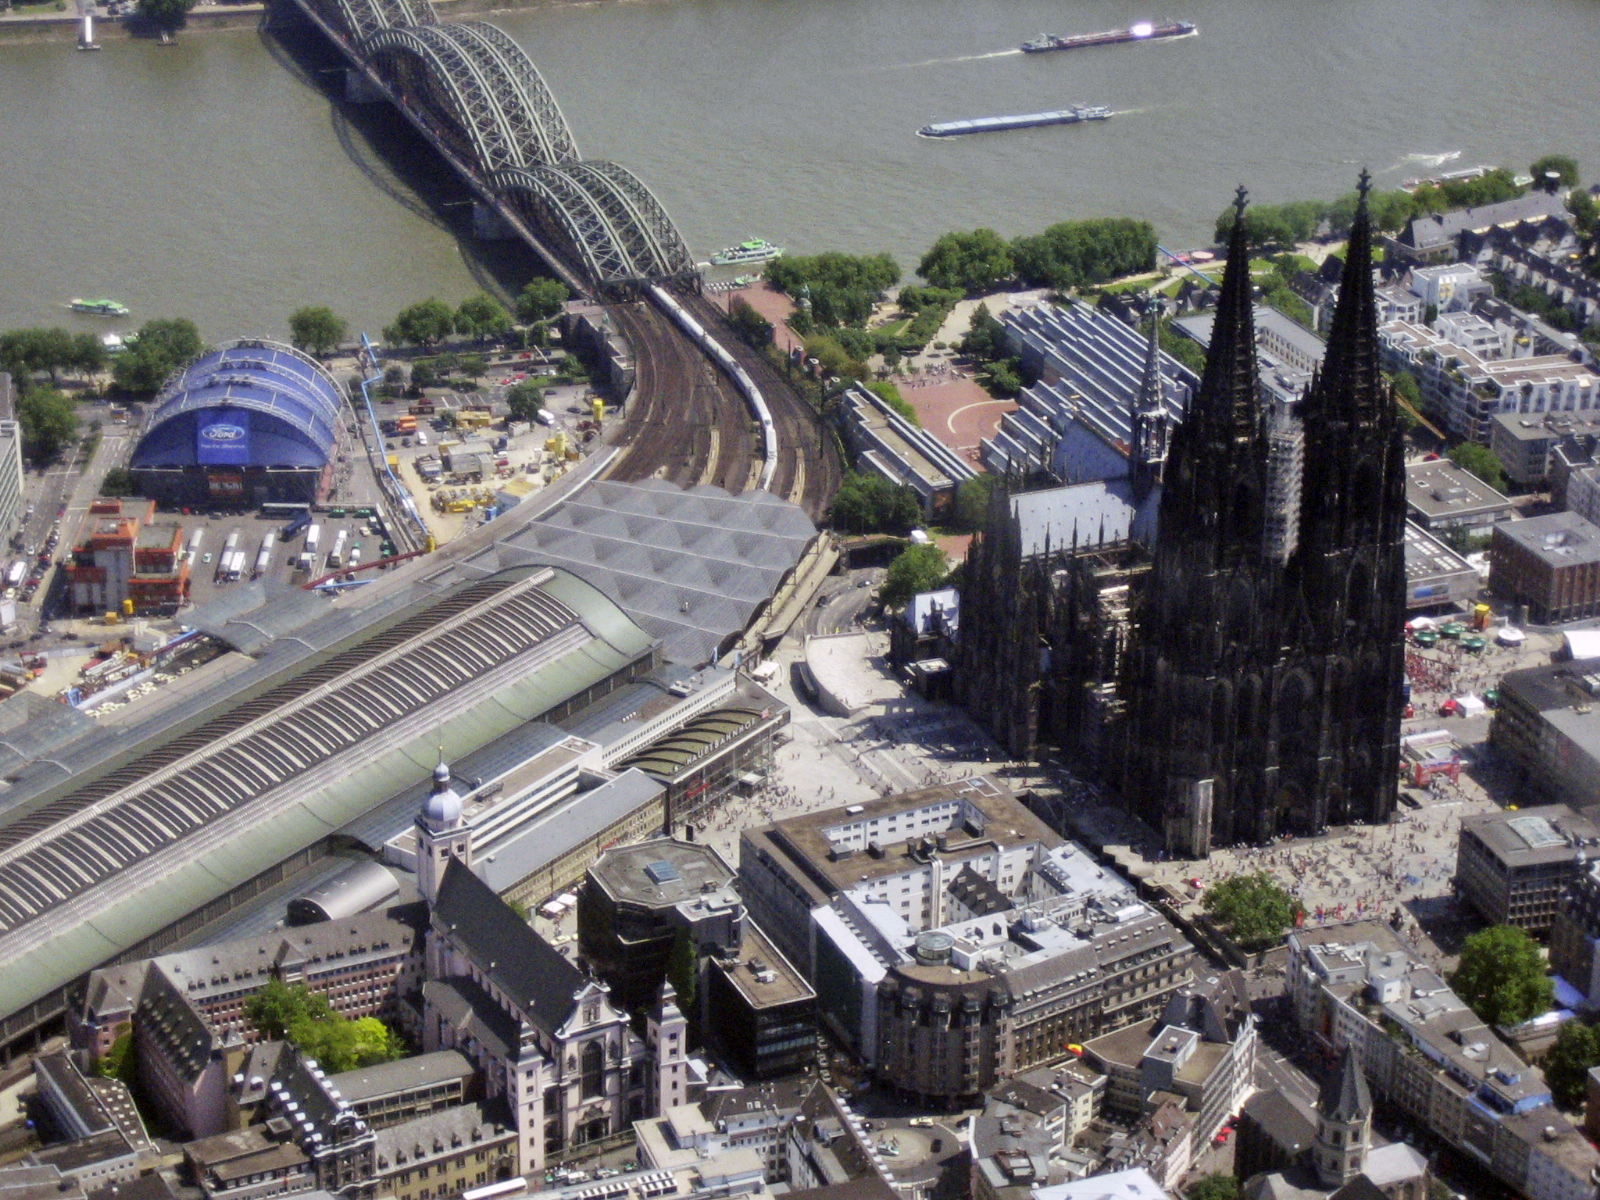
\includegraphics[width=0.45\linewidth]{Abbildungen/Koeln_RdFlug_1}}
\caption{Zwei Abbildungen}
\label{fig:zweiAbbildungen}
\end{figure}

\blindtext[2]

\begin{table}
    \centering
    \begin{tabular}{|>{\bfseries\footnotesize\centering}p{4cm}|c|r|}
        \hline
                                      & \multicolumn{2}{c|}{Werte} \\
        \cline{2-3}
        Stichproben-ID & Wert 1   & Wert 2\\
        \hline
        1                            & 1.00323 & 0.43\\
        2                            & 12.3        & 3.4\\
        \blindtext           & 1.2          & 0.34343\\
        \hline
    \end{tabular}
    \caption{Eine erste Tabelle}
    \label{tab:ersteTabelle}
\end{table}

\blindtext
\begin{table}
    \centering
    \sisetup{
        table-number-alignment=center,
        table-figures-integer=2,
        table-figures-decimal=3,
        output-decimal-marker={,},
        table-auto-round
        }
    \begin{tabular}{>{\bfseries\footnotesize\centering}p{4cm}SS}
        \toprule
        & \multicolumn{2}{c}{Werte} \\
        \cmidrule(lr){2-3}
        Stichproben-ID & {Wert 1}   & {Wert 2}\\
        \midrule
        1                            & 1.00323 & 0.43\\
        2                            & 12.3        & 3.4\\
        3                            & 1.2          & 0.34343\\
        \bottomrule
    \end{tabular}
    \caption{Eine erste Tabelle}
    \label{tab:ersteTabelleBooktabs}
\end{table}

\blindtext[3]
\begin{table}
    \centering
%    \begin{tabularx}{0.8\linewidth}{|>{\bfseries\footnotesize\centering}X|c|r|}
    \begin{tabularx}{\linewidth}{|>{\bfseries\footnotesize\centering}p{4cm}|X|X|}
        \hline
        & \multicolumn{2}{c|}{Werte} \\
        \cline{2-3}
        Stichproben-ID & Wert 1   & Wert 2\\
        \hline
        1                            & 1.003234646464 & 0.43\\
        2                            & 12.3        & 3.4\\
        \blindtext           & 1.2          & 0.34343\\
        \hline
    \end{tabularx}
    \caption{Eine erste Tabelle}
    \label{tab:ersteTabelle}
\end{table}

\chapter{Mathematik}
\section{Fließtext}
Sei a>0

Sei $a>0$ und $b\leq 1$

\begin{equation}\label{eq:einfacheFormel}
a+b\leq c
\end{equation}

Die Ungleichung~\eqref{eq:einfacheFormel} \ldots{}

Seien $a,b,c,d,e,f,g,h,i \in \mathbb{R}$. Dann gilt:
\[
a+b\leq c + \left(\frac{d}{e+f}\right)^{2+i} + \sqrt{\frac{g}{h+i}}
\]

\[
\bigl((2+3)\cdot 5\bigr)
\]

\begin{equation}
\begin{split}
a+b&\leq c\\
       &= d+e\\
       &\leq d+(f+g)\\
\end{split}
\end{equation}

\begin{align}
a+b&\leq c\\
       &= d+e\\
       &\leq d+(f+g)
\end{align}

\[
\log(x)=2\max_{x\in \mathbb{R}}x^3\lim_{x\to-\infty}e^x
\]

\begin{definition}[Arithmetisches Mittel]
    Seien Messwerte $x_1,\ldots,x_N$ gegeben. Dann heißt
    \begin{equation}
    \bar{x}=\frac{1}{N}\sum_{i=1}^{N}x_i
    \end{equation}
    das arithmetische Mittel.
\end{definition}

\section{Literatur}
Wie bereits \autor{Herbert Voß} in \cite[12--16]{Voss.2012}, aber auch in \cite[34]{Voss.2007} schreibt,

\cite{Mosgen.1998}

\cite{Mittelbach.2004}

\fbox{\parbox[t]{0.4\textwidth}{\blindtext[2]}}\hspace*{\fill}
\fbox{\parbox[t]{0.4\textwidth}{\blindtext}}\\

A B\hfill B\\
\newlength{\myheight}
\settoheight{\myheight}{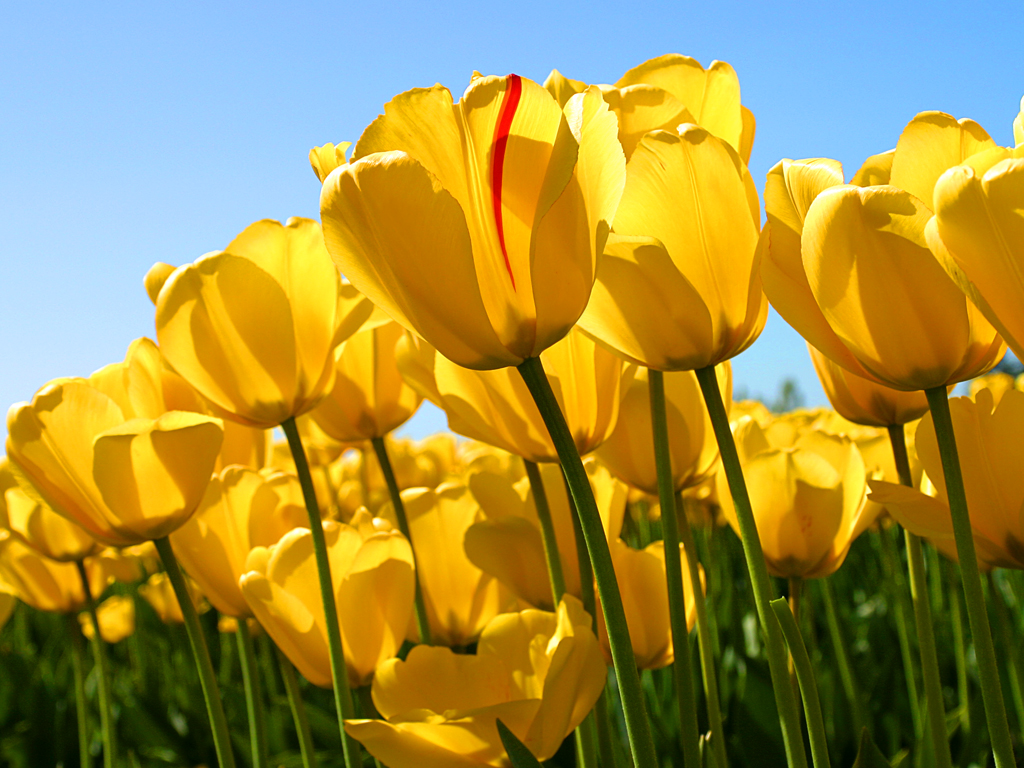
\includegraphics[width=2cm]{Abbildungen/Tulips}}
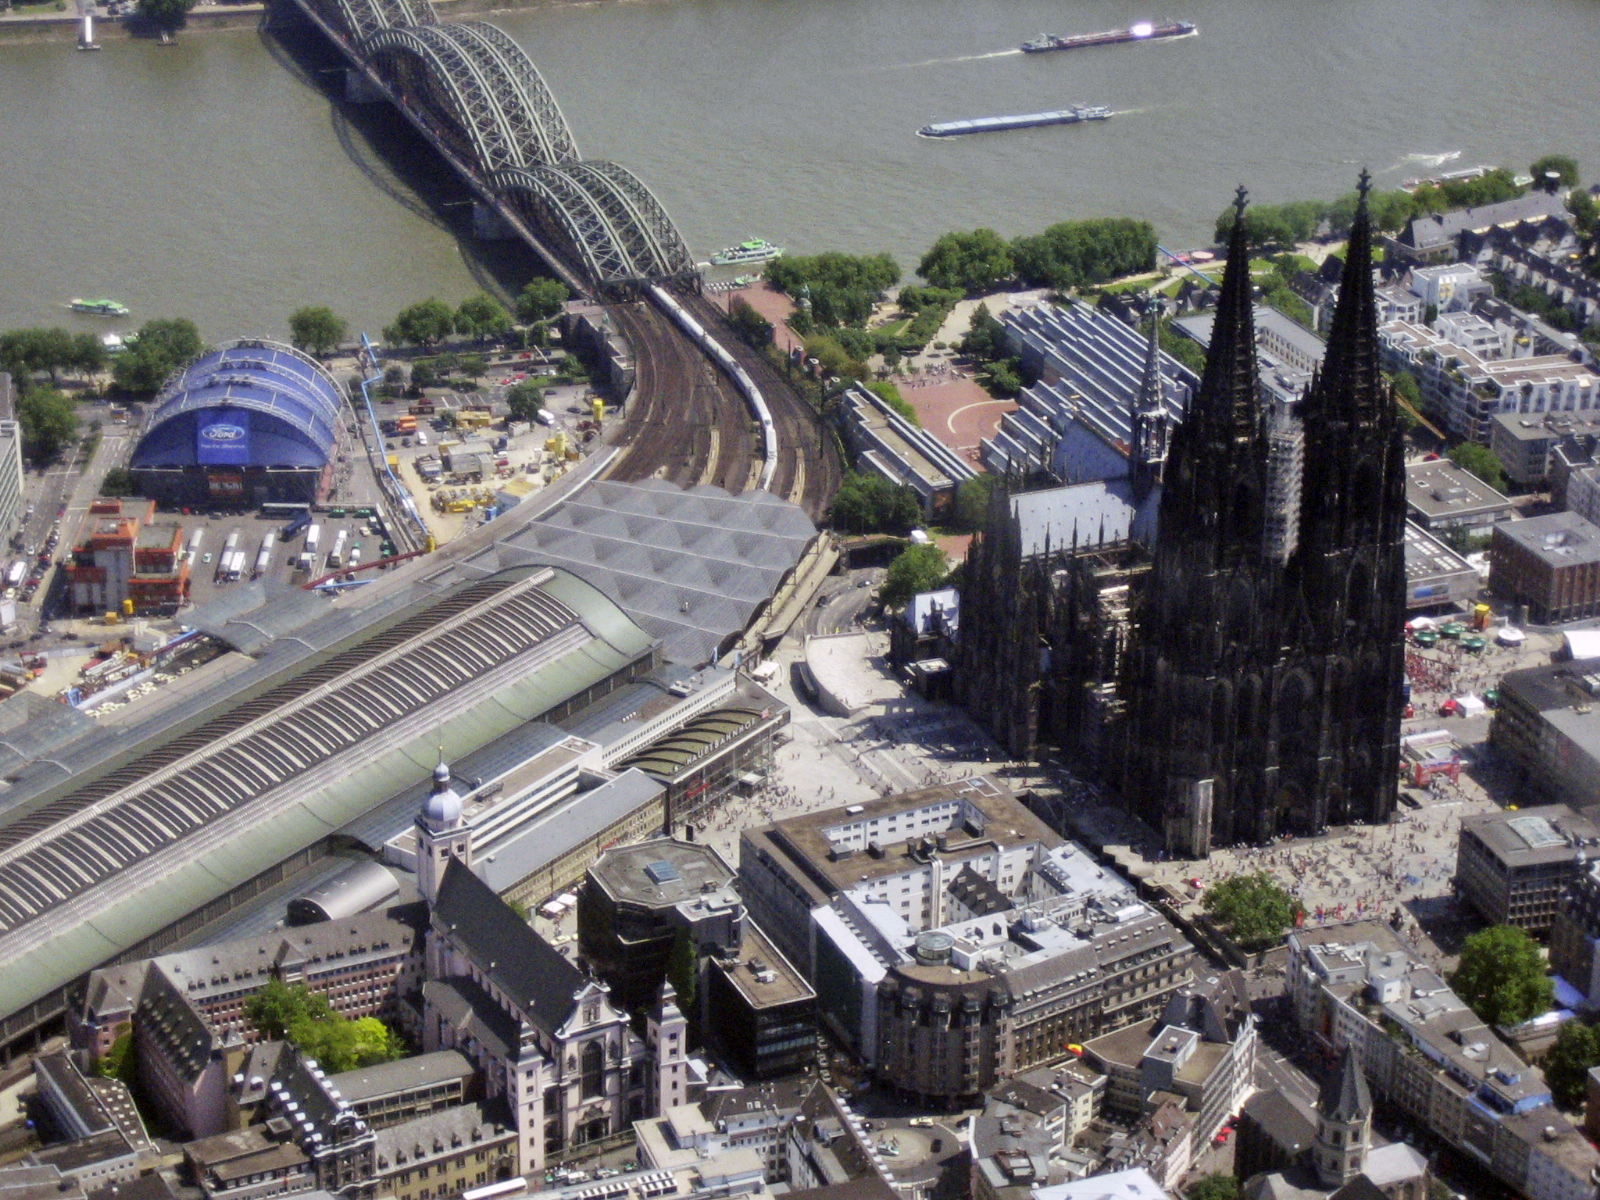
\includegraphics[height=\myheight]{Abbildungen/Koeln_RdFlug_1}
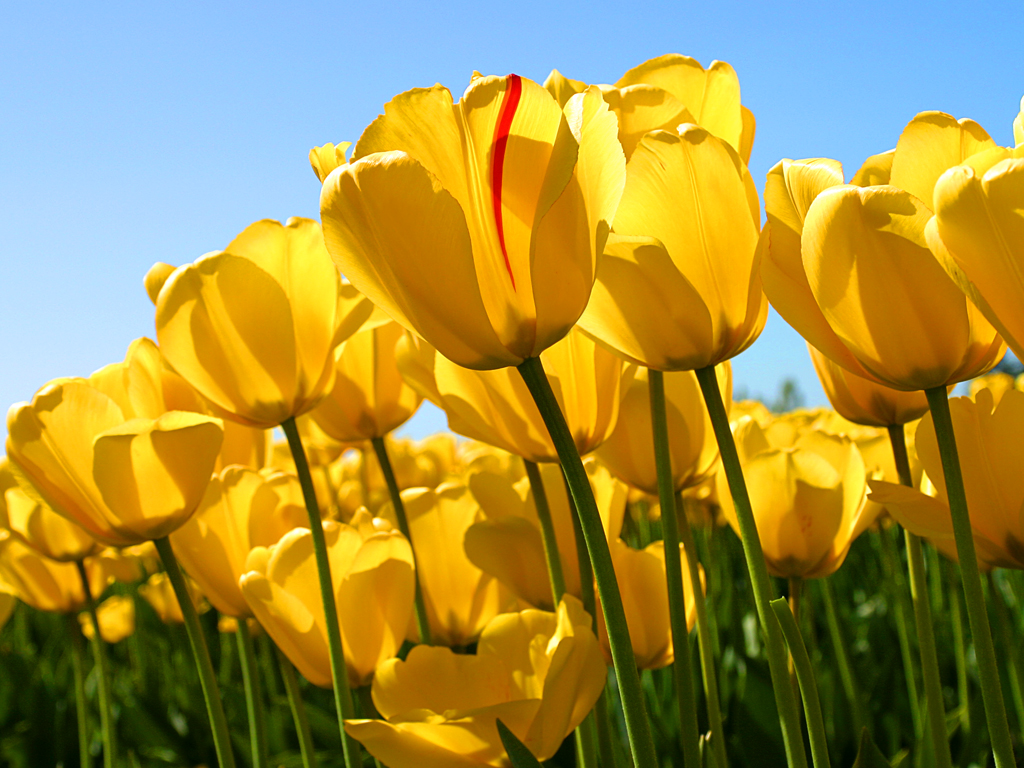
\includegraphics[width=2cm]{Abbildungen/Tulips}

\addtolength{\myheight}{3cm}
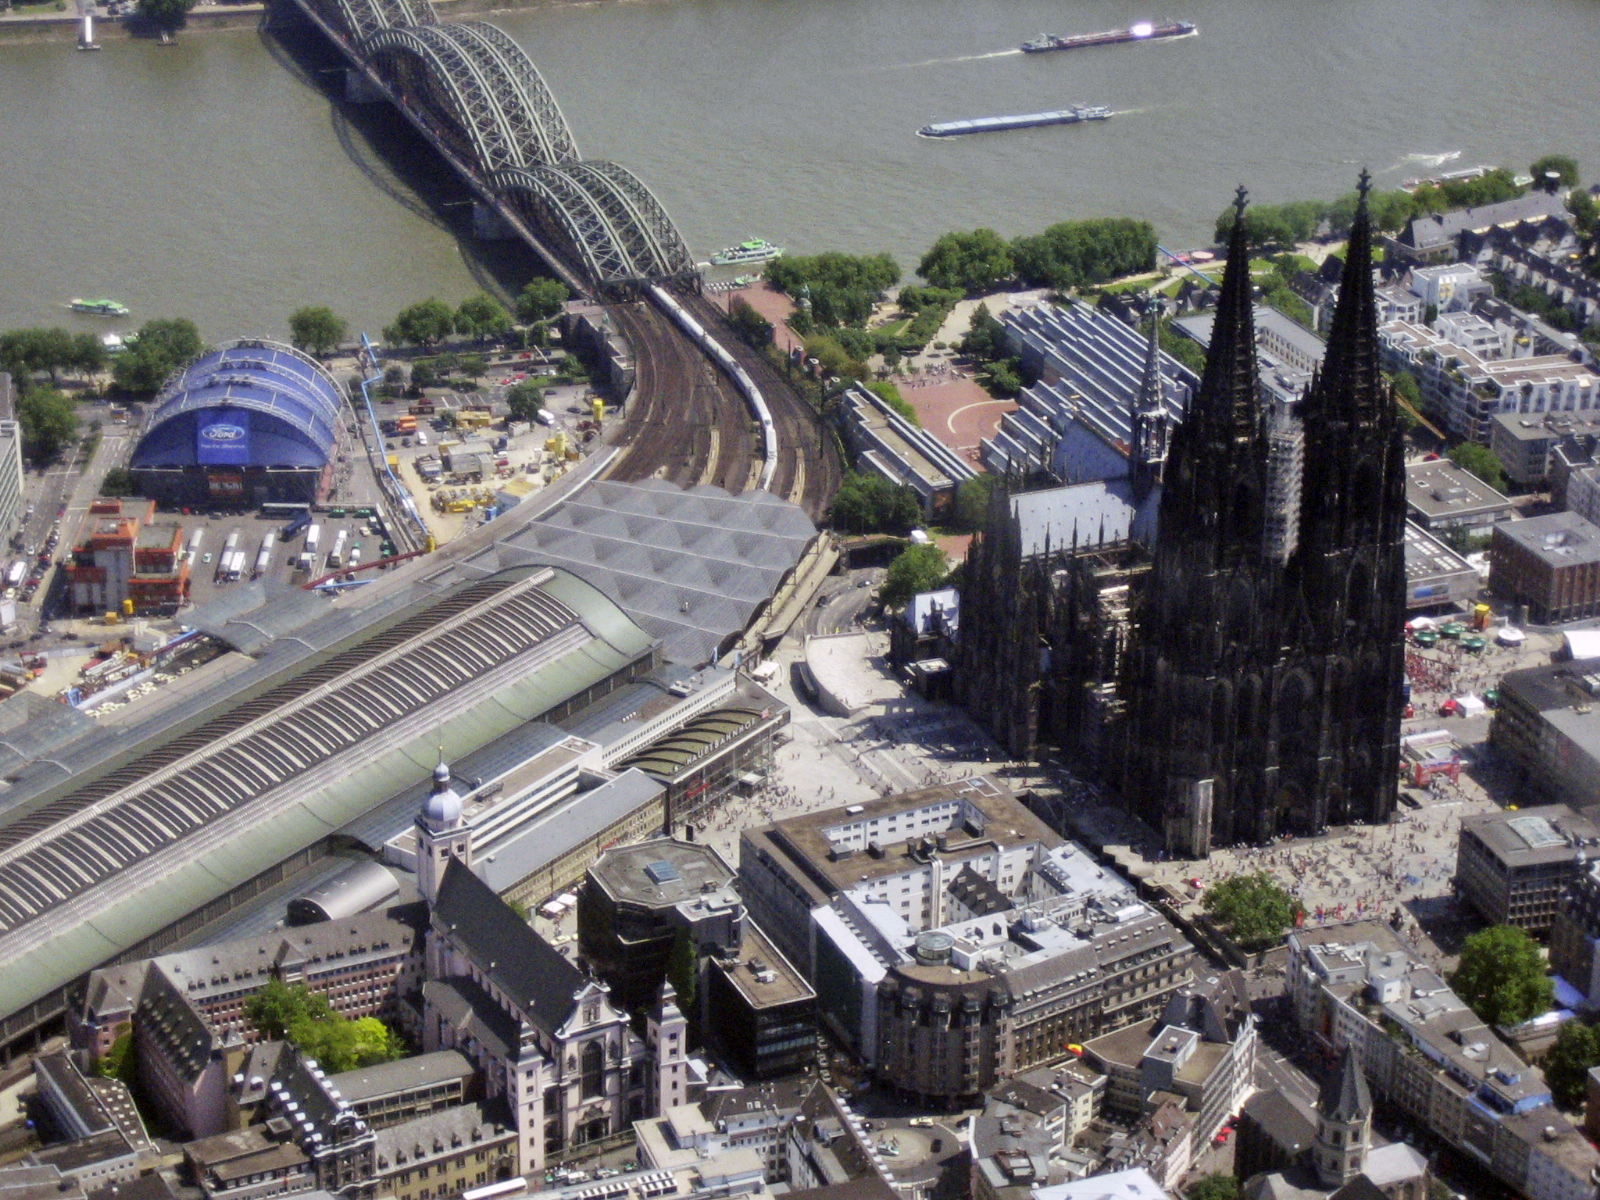
\includegraphics[height=\myheight]{Abbildungen/Koeln_RdFlug_1}

\nocite{*}
\printbibliography[nottype=online]
\printbibliography[type=online]
\end{document}